%----------------------------------------------------------------------------------------
%	PACKAGES AND OTHER DOCUMENT CONFIGURATIONS
%----------------------------------------------------------------------------------------

\documentclass[twoside,twocolumn,a4paper]{article}

\usepackage{blindtext} % Package to generate dummy text throughout this template 

\usepackage{mhchem}

\usepackage{gensymb}

\usepackage[super]{natbib}

\usepackage[T1]{fontenc} % Use 8-bit encoding that has 256 glyphs

\usepackage{lmodern}

\usepackage[hyphenbreaks]{breakurl}

\usepackage[hyphens]{url}

%\usepackage[super,sort&compress]{natbib}
%\usepackage{natbib}
%\setlength{\bibsep}{0.0pt}

\usepackage{graphicx}

\linespread{1.05} % Line spacing - Palatino needs more space between lines
\usepackage{microtype} % Slightly tweak font spacing for aesthetics

\usepackage[spanish]{babel} % Language hyphenation and typographical rules

\usepackage[numbib,notlof,notlot,nottoc]{tocbibind} % Shows bibliography as a section

\usepackage[hmarginratio=1:1,top=32mm,columnsep=20pt]{geometry} % Document margins

\usepackage[hang, small,labelfont=bf,up,textfont=up]{caption} % Custom captions under/above floats in tables or figures

\usepackage[section]{placeins}

\usepackage{float}

\usepackage{booktabs} % Horizontal rules in tables

\usepackage{enumitem} % Customized lists

\setlist[itemize]{noitemsep} % Make itemize lists more compact

\usepackage{abstract} % Allows abstract customization

\renewcommand{\abstractnamefont}{\normalfont\bfseries} % Set the "Abstract" text to bold

\usepackage{fancyhdr} % Headers and footers
\pagestyle{fancy} % All pages have headers and footers
\fancyhead{} % Blank out the default header
\fancyfoot{} % Blank out the default footer
\fancyhead[C]{Laboratorio 4 $\bullet$ Informe 2 $\bullet$ Grupo 3: Poggi, R\'ios Ch\'avez} % Custom header text
\fancyfoot[C]{\thepage} % Custom footer text

\usepackage{titling} % Customizing the title section

\usepackage{hyperref} % For hyperlinks in the PDF

%----------------------------------------------------------------------------------------
%	TITLE SECTION
%----------------------------------------------------------------------------------------

\setlength{\droptitle}{-4\baselineskip} % Move the title up

\pretitle{\begin{center}\LARGE\bfseries} % Article title formatting
\posttitle{\end{center}} % Article title closing formatting
\title{Difusividad t\'ermica} % Article title
\author{%
\textsc{Ignacio Poggi} \\[1ex] % Your name
\normalsize \href{mailto:ignaciop.3@gmail.com}{ignaciop.3@gmail.com} % Your email address
\and % Uncomment if 2 authors are required, duplicate these 4 lines if more
\textsc{Carlos R\'ios Ch\'avez} \\[1ex] % Second author's name
\normalsize \href{mailto:carlos_rios_ch@hotmail.com}{carlos\_rios\_ch@hotmail.com} % Second author's email address
}



\date{Grupo 3 - Laboratorio 4, C\'atedra Schmiegelow - Departamento de F\'isica, Facultad de Ciencias Exactas y Naturales, Universidad de Buenos Aires \newline \\ \today} % Leave empty to omit a date
\renewcommand{\maketitlehookd}{%
\begin{abstract}
\noindent En este trabajo se estudi\'o la  difusi\'on  del  calor utilizando una barra de cobre sometida a una fuente peri\'odica, modulada por una onda cuadrada en uno de sus extremos. Se calcul\'o la velocidad y el coeficiente de decaimiento de la onda de calor en el estado estacionario, obteniendo experimentalmente la constante de difusividad t\'ermica del \ce{_{29}Cu}, $\kappa = (2,46 \pm 0,70)*10^{-4} \frac{m^{2}}{seg}$.

\end{abstract}
}

%----------------------------------------------------------------------------------------

\begin{document}
\maketitle

% Print the title

%----------------------------------------------------------------------------------------
%	ARTICLE CONTENTS
%----------------------------------------------------------------------------------------

\section{Introducci\'on}

En un s\'olido is\'otropo y homog\'eneo, cuya difusividad t\'ermica $\kappa$ es independiente de la temperatura, la ecuaci\'on que determina el comportamiento t\'ermico es\cite{eq:calor}:

\begin{equation}
\label{eq:calor}
\frac{\partial^2 \theta (x,t)}{\partial x^{2}} = \frac{1}{\kappa} \frac{\partial \theta (x,t)}{\partial t}
\end{equation}

siendo $\theta(x,t)$ la temperatura en la posici\'on $x$ a tiempo $t$. A la ecuaci\'on (\ref{eq:calor}) se la conoce como la ecuaci\'on de Fourier unidimensional. Para determinar las condiciones de contorno que corresponden a nuestro experimento, se dispuso en el origen de la barra una fuente de calor peri\'odica, lo que permite expresar $\theta(x,t)$ en este extremo de la siguiente manera:

\begin{equation}
\label{eq:theta0}
\theta(0,t) = \sum_{n = 1, 3, 5, ...}^{\infty} \frac{4\theta_{0}}{n\pi} sen(\frac{2n\pi t}{\tau})
\end{equation}

Adem\'as, como la barra se supone semi-infinita, la condici\'on en el otro extremo ser\'a $\theta(\infty,t) = 0$; es decir, se considera que la temperatura al final de la barra decae completamente. \newline

\par
Siendo que nos interesa la distribuci\'on de temperatura en el r\'egimen estacionario, se propone la siguiente serie de Fourier como soluci\'on a la ecuaci\'on (\ref{eq:calor}):

\begin{equation}
\label{eq:solgeneral}
\theta(x,t) = \sum_{n = 1}^{\infty} A_{n}(x) sen(\omega_{n}t - k_{n}x)
\end{equation}

donde $A_{n}$, $\omega_{n}$ y $k_{n}$ son la amplitud, frecuencia y el n\'umero de onda del $n$-\'esimo arm\'onico. Reemplazando la ecuaci\'on (\ref{eq:solgeneral}) en (\ref{eq:calor}), junto a las condiciones de contorno mencionadas en (\ref{eq:theta0}) y $\theta(\infty,t) = 0$, se obtiene la soluci\'on para el sistema estudiado:

\begin{equation}
\label{eq:solbarra}
\theta(x,t) = \sum_{n = 1, 3, 5, ...}^{\infty} \theta_{n}e^{\epsilon_{n}x} sen(\omega_{n}t - \epsilon_{n}x)
\end{equation}

donde

\begin{equation}
\label{eq:conds}
\theta_{n} = \frac{4\theta_{0}}{n\pi}, \omega_{n} = \frac{2n\pi t}{\tau}, \epsilon_{n} = \sqrt{\frac{\omega_{n}}{2\kappa}}
\end{equation}


Se puede ver que, a medida que aumenta $n$, los arm\'onicos se desvanecen r\'apidamente dado que $\epsilon_{n}$ aumenta con la frecuencia. Debido a esto, es posible aproximar a la distribuci\'on de temperatura en puntos lo suficientemente alejados del origen de la barra, utilizando solamente el primer arm\'onico:

\begin{equation}
\label{eq:firstharmonic}
\theta(x,t) \approx A_{0}e^{\epsilon x} cos(\omega(t - \frac{x}{v}))
\end{equation}

escogiendo el origen de tiempo tal que $\theta$ es m\'aximo en $ x = 0$. Considerando la ecuaci\'on (\ref{eq:firstharmonic}) y el primer arm\'onico de la soluci\'on completa (\ref{eq:solbarra}), se pueden obtener las expresiones:

\begin{equation}
\label{eq:ke}
\kappa_{\epsilon} = \frac{\pi}{\tau \epsilon^{2}}
\end{equation}

\begin{equation}
\label{eq:kv}
\kappa_{v} = \frac{v^{2} \tau}{4\pi}
\end{equation}


que relacionan las propiedades t\'ermicas del material, en este caso la difusividad t\'ermica $\kappa$, con dos propiedades de la onda: la velocidad $v$ y el coeficiente de decaimiento $\epsilon$. \newline

\par
Finalmente, combinando las ecuaciones (\ref{eq:ke}) y (\ref{eq:kv}), se obtiene una expresi\'on para el coeficiente de difusividad t\'ermica del cobre en funci\'on de los par\'ametros $v$ y $\epsilon$, determinados experimentalmente:

\begin{equation}
\label{eq:kappa}
\kappa = \frac{v}{2\epsilon}
\end{equation}

la cual permite comparar el valor de $\kappa$ experimental con el te\'orico \cite{teo:kappa} de $\kappa = 1,12*10^{-4}$ $\frac{m^{2}}{seg}$

%------------------------------------------------

\section{Dispositivo experimental}

Los instrumentos de laboratorio utilizados fueron:
\begin{itemize}
\item 
\label{Laser} PC con software MATLAB para la adquisici\'on y an\'alisis de los datos.
\item Mult\'imetro Agilent 34970A.
\item Multiplexor de 8 canales.
\item Barra de cobre de 1,5 $\pm$ 0,1 cm de di\'ametro y 50,0 $\pm$ 0,1 cm de largo.
\item Siete termocuplas (2 de tipo K y 5 de tipo J).
\item Soldador.
\item Contactor.
\item Generador de funciones Tektronix AFG3021B.
\end{itemize}

Se dispuso un soldador conectado a un contactor controlado por un generador de ondas, el cual se configur\'o para emitir una onda cuadrada de per\'iodo $\tau$ = 170 seg. durante los r\'egimenes transitorio y estacionario. Luego, la punta del soldador fue insertada en uno de los extremos de la barra aislada, y a los 10 minutos se comenz\'o a medir el r\'egimen transitorio. \newline

\par
Las medidas de la temperatura se obtuvieron mediante 7 termocuplas de tipo K y J, insertadas a lo largo de la barra en diferentes posiciones como muestra la siguiente tabla (todos los valores tomando como posici\'on 0 al extremo fijado al soldador):

\begin{table}[H]
\centering
\caption{Posici\'on de cada termocupla en la barra con respecto al extremo en contacto con el soldador (posici\'on 0).}
\label{tab:posiciones}
\begin{tabular}{|c|c|}
\hline
Termocupla & Posici\'on ( $\pm 0,1 cm$) \\ \hline
1 K & 4,1\\ \hline
2 K & 8,6\\ \hline
3 J & 13,4\\ \hline
4 J & 17,1\\ \hline
5 J & 22,0\\ \hline
6 J & 29,2\\ \hline
7 J & 36,4\\ \hline
\end{tabular}
\end{table}


Estas termocuplas se conectaron a un multiplexor, el cual fue conectado a un mult\'imetro de 8 canales, con el que se realiz\'o la adquisici\'on de los datos utilizando 7 de ellos. En la siguiente figura se puede ver un esquema del dispositivo utilizado:

\begin{figure}[H]
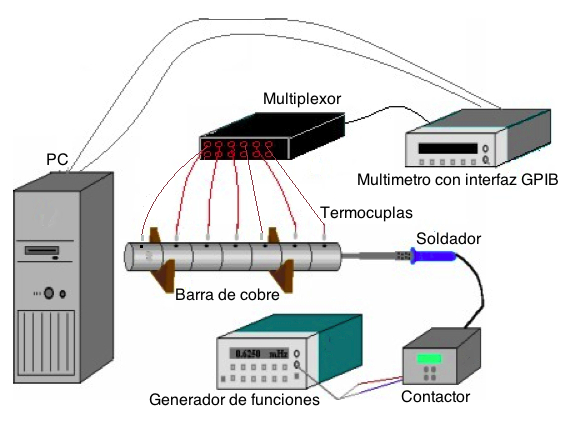
\includegraphics[width=\linewidth]{dispexp.jpg}
\caption{Dispositivo experimental. Cabe destacar que la barra de cobre se encuentra aislada con una capa interna de espuma aislante y una externa de PVC.}
\label{fig:disenoestatico}
\end{figure}

Mediante un programa realizado en MATLAB; el cual se utilizo para configurar al mult\'imetro v\'ia interfaz GPIB, se tomaron 1000 mediciones secuenciales en las termocuplas cada 5 segundos, es decir; se obtuvieron 7 valores de temperatura (una por cada termocupla) cada 5 segundos; esto equivale a una medici\'on. Este paso se repiti\'o durante un tiempo total de 5000 segundos (aproximadamente 1:30 hs.), primero para el r\'egimen transitorio y luego para el estacionario; dejando pasar para este \'ultimo 3 horas desde el comienzo de la medici\'on del transitorio. \newline

\par
Luego, se obtuvieron todos los datos guardados en el mult\'imetro con el mismo programa en MATLAB, para su posterior an\'alisis.

%------------------------------------------------
\section{Resultados y an\'alisis}

Para estimar la temperatura a la cual el sistema alcanza el r\'egimen estacionario, se aliment\'o al soldador con una onda cuadrada de per\'iodo $\tau$ = 170 seg. y amplitud de 6,432 Vpp. durante la primera medici\'on realizada en un tiempo de 1:30 hs.; observando que la misma aumenta de manera uniforme durante \'este r\'egimen hasta oscilar alrededor de un valor fijo en cada termocupla para los \'ultimos valores de tiempo en esta medici\'on ($t \approx$ 4800 a 5000 seg.), teniendo en cuenta el error de precisi\'on de las mismas ($\pm$ 1,5 \degree C). Por ejemplo, en las termocuplas 1 y 4, $T_{Ch 1}$ = 89,5 \degree C y $T_{Ch 4}$ = 79,2 \degree C respectivamente, como puede verse en la siguiente figura.

\begin{figure}[H]
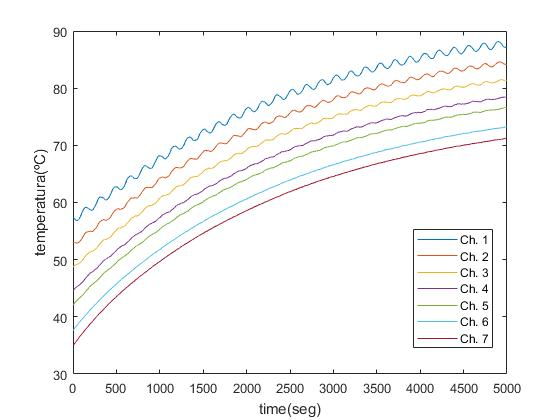
\includegraphics[width=\linewidth]{Tvst_transitorio.jpg}
\caption{Valores de temperatura en cada termocupla durante el regimen transitorio}
\label{fig:Tvst_transitorio}
\end{figure}


Luego, se deja evolucionar al sistema durante 3 horas m\'as, para poder alcanzar el r\'egimen estacionario, y se realiza la segunda medici\'on, con los mismos par\'ametros de per\'iodo y amplitud que para el transitorio.

FIGURA DEL ESTACIONARIO ACA?????

Podemos notar que la temperatura inicial de la termocupla 1 es de 91.5 \degree C, muy cercano al valor de la \'ultima medici\'on de temperatura (a $t$ = 5000 seg) para el r\'egimen transitorio. Teniendo en cuenta esto, m\'as el rango de precisi\'on mencionado en cada termocupla; nos indica que el tiempo de 3 horas utilizado para alcanzar el r\'egimen estacionario una vez comenzado el experimento fue el correcto.

\subsection{C\'alculo de la velocidad $v$ y la constante de decaimiento $\epsilon$ de la onda t\'ermica}


$\kappa_{\epsilon} = (4,97 \pm 0,8) * 10^{-4} \frac{m^{2}}{seg}$ 

$\kappa_{v} = (1,24 \pm 0,8) * 10^{-4} \frac{m^{2}}{seg}$

Aunque el valor estimado de $\kappa$ puede ser calculado mediante el promedio de $\kappa_{\epsilon}$ y $\kappa_{v}$; en nuestro caso ....; existe una pequena diferencia de 0.7 con el obtenido mediante la ecuacion v/2e = TANTO.

Lo ideal seria que estos dos valores den muy proximos entre si, para minimizar el error en el calculo. En nuestro caso, al calcular las temperaturas medias, se indujo un error bla bla bla.

Se obtuvo una diferencia del 45 por ciento en el calculo de k con respecto al valor tabulado de k = 1,12.



%------------------------------------------------

\section{Conclusiones}


%----------------------------------------------------------------------------------------
%	REFERENCE LIST
%----------------------------------------------------------------------------------------
\newpage
\begin{thebibliography}{99} % Bibliography - this is intentionally simple in this template


\bibitem{eq:calor} A. Bodas, V. G\'andia and E. L\'opez-Baeza, \textit{An undergraduate experiment on the propagation of thermal waves}, American Journal of Physics, \textbf{66}, 528 (1998).

\bibitem{teo:kappa} W. Czarnetzki, M. Wandelt, and W. Roetzel, \textit{Thermal wave analysis for measurements of thermal diffusivity, Proceedings of the Joint Conference 1996: IEEE Instrumentation and Measurement Technology Conference and IMEKO Technical Committee 7}, Brussels, Belgium, 4-6 June 1996 (IEEE, New York, 1996), p\'ag. 1195.
 
\end{thebibliography}


%----------------------------------------------------------------------------------------

\end{document}